Consider the following feedback system
\begin{center}
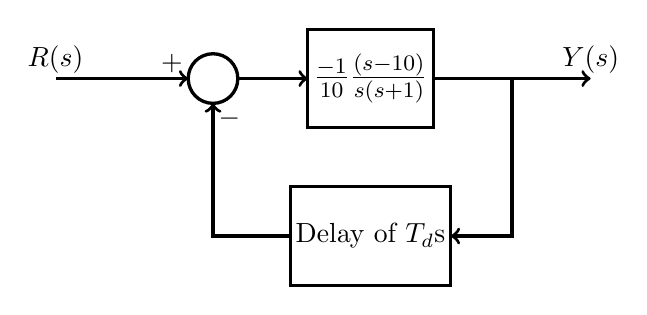
\begin{tikzpicture}[scale=1,inner sep=0pt,outer sep=0pt,very thick,
sysblock/.style={draw,rectangle,inner sep=2pt,minimum width=1.25cm,minimum height=1.25cm,very thick}]
\draw (2,0) node[draw,circle] (sum1) {$\rule{0pt}{18pt}$};
\draw (4,0) node[sysblock] (G) {\large$\frac{-1}{10}\frac{(s-10)}{s(s+1)}$};
\draw (4,-2) node[sysblock] (D) {Delay of $T_{d}$s};
\draw[->] (0,0) node[above=2pt] {$R(s)$} -- (sum1.180) node[above left=2pt] {$+$};
\draw[->] (sum1.0) --  (G);
\draw[->] (G.0) -- ++(2,0) node[above=2pt] {$Y(s)$};
\draw[->] (G.0) ++(1,0) |- (D.0);
\draw[->] (D.180)  -| (sum1.-90) node[below right=2pt] {$-$};
\end{tikzpicture}
\end{center}
 (a) Sketch the Bode plot for the open loop system (i.e. the loop gain) assuming $T_{d}=0$. For full credit, scale the x and y axes and indicate the magnitude and phase at every break point. (b)  From your sketch, determine the maximum value of $T_{d}>0$ that can be tolerated before the closed loop system becomes unstable.
\begin{center}
\includegraphics[width=6in]{\mainfolder/LectureNotes/\lecturefolder/HomeworkProblems/Problem04/blankbode.pdf}
\end{center}
